\documentclass[tikz,border=10pt]{standalone}
\usepackage{pgfplots}
\pgfplotsset{compat=1.18}
\newcommand{\flashspread}{\textsc{FlashSpread}}

\begin{document}
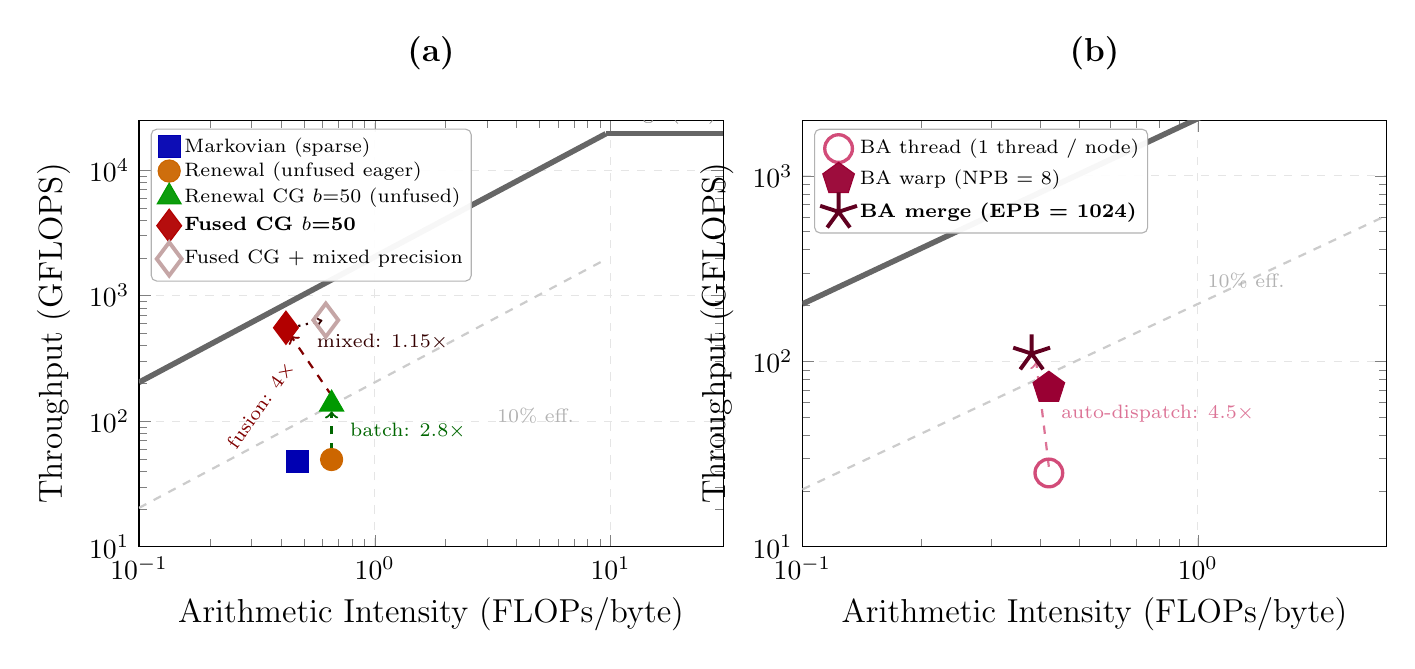
\begin{tikzpicture}

% ============================================================
% LEFT PANEL: regular-graph fusion / batching progression.
% ============================================================
\begin{axis}[
    name=panelA,
    width=9cm, height=7cm,
    xmode=log, ymode=log,
    log basis x=10, log basis y=10,
    xmin=0.1, xmax=30,
    ymin=10, ymax=25000,
    grid=major, grid style={dashed,gray!20},
    xlabel={Arithmetic Intensity (FLOPs/byte)},
    ylabel={Throughput (GFLOPS)},
    xlabel style={font=\large}, ylabel style={font=\large},
    xticklabel style={font=\normalsize},
    yticklabel style={font=\normalsize},
    title={(a)},
    title style={font=\large\bfseries, yshift=0.3cm},
    legend style={
        at={(0.02,0.98)}, anchor=north west,
        legend cell align=left, font=\scriptsize,
        fill=white, fill opacity=0.95, draw=black!30,
        text opacity=1, rounded corners=2pt,
        inner sep=2pt, nodes={inner sep=1pt},
    },
]

% A100 ceilings.
\addplot[domain=0.1:9.56, samples=50, color=black!60, line width=2pt, forget plot] {2039 * x};
\addplot[domain=9.56:30, samples=10, color=black!60, line width=2pt, forget plot] {19500};
\node[font=\scriptsize, text=black!50, anchor=south west] at (axis cs:9.56,19500) {ridge (9.6)};
\addplot[domain=0.1:9.56, samples=50, color=gray!40, line width=0.8pt, dashed, forget plot] {2039 * x * 0.1};
\node[font=\scriptsize, text=gray!60, anchor=south west] at (axis cs:3,80) {10\% eff.};

% Data points.
\addplot[only marks, mark=square*, mark size=4pt, color=blue!70!black,
         mark options={fill=blue!70!black}]
         coordinates {(0.469, 47.6)};
\addplot[only marks, mark=*, mark size=4pt, color=orange!80!black,
         mark options={fill=orange!80!black}]
         coordinates {(0.656, 49.5)};
\addplot[only marks, mark=triangle*, mark size=5pt, color=green!60!black,
         mark options={fill=green!60!black}]
         coordinates {(0.656, 137.0)};
\addplot[only marks, mark=diamond*, mark size=6pt, color=red!70!black,
         mark options={fill=red!70!black}]
         coordinates {(0.42, 555)};
% Fused CG + mixed precision (Section 5.7): narrower per-tensor
% storage (state int8, age fp16, infectivity/weights bf16; fp32
% accumulator) cuts per-step bytes by ~32% without changing the
% FLOPs count, shifting the kernel's operating point to higher AI
% and higher achieved GFLOPS. Values derived from the baseline
% Fused CG point and the measured 1.15x events/s lift on ER d=8,
% N=1e6 (Table 6, Figure 6 left panel).
\addplot[only marks, mark=diamond, mark size=6pt, color=red!35!black!35!white,
         line width=1.4pt]
         coordinates {(0.62, 638)};

% Inline marker labels removed — the legend already identifies each
% point. Removing them also declutters the panel around the
% fusion/mixed arrows and makes the 2x2 progression easier to read.

\draw[->, thick, red!50!black, dashed]
    (axis cs:0.656, 160) -- (axis cs:0.44, 480)
    node[midway, anchor=south east, font=\scriptsize, text=red!50!black, rotate=55]
    {fusion: $4\times$};
\draw[->, thick, green!40!black, dashed]
    (axis cs:0.656, 58) -- (axis cs:0.656, 120)
    node[midway, anchor=west, font=\scriptsize, text=green!40!black, xshift=3pt]
    {batch: $2.8\times$};
% Mixed-precision arrow: up-and-right from Fused CG to the new point.
\draw[->, thick, red!20!black, dotted]
    (axis cs:0.44, 555) -- (axis cs:0.60, 635)
    node[midway, anchor=north west, font=\scriptsize, text=red!20!black]
    {mixed: $1.15\times$};

\legend{
    Markovian (sparse),
    Renewal (unfused eager),
    Renewal CG $b$=50 (unfused),
    \textbf{Fused CG $b$=50},
    Fused CG + mixed precision
}

\end{axis}

% ============================================================
% RIGHT PANEL: zoomed degree-heterogeneous regime (Barabasi-Albert).
% ============================================================
\begin{axis}[
    at={(panelA.right of south east)}, anchor=south west, xshift=10mm,
    width=9cm, height=7cm,
    xmode=log, ymode=log,
    log basis x=10, log basis y=10,
    xmin=0.1, xmax=3,
    ymin=10, ymax=2000,
    grid=major, grid style={dashed,gray!20},
    xlabel={Arithmetic Intensity (FLOPs/byte)},
    ylabel={Throughput (GFLOPS)},
    xlabel style={font=\large}, ylabel style={font=\large},
    xticklabel style={font=\normalsize},
    yticklabel style={font=\normalsize},
    title={(b)},
    title style={font=\large\bfseries, yshift=0.3cm},
    legend style={
        at={(0.02,0.98)}, anchor=north west,
        legend cell align=left, font=\scriptsize,
        fill=white, fill opacity=0.95, draw=black!30,
        text opacity=1, rounded corners=2pt,
        inner sep=2pt, nodes={inner sep=1pt},
    },
]

\addplot[domain=0.1:3, samples=50, color=black!60, line width=2pt, forget plot] {2039 * x};
\addplot[domain=0.1:3, samples=50, color=gray!40, line width=0.8pt, dashed, forget plot] {2039 * x * 0.1};
\node[font=\scriptsize, text=gray!60, anchor=south west] at (axis cs:1,220) {10\% eff.};

\addplot[only marks, mark=o, mark size=5pt, color=purple!70, line width=1.2pt]
    coordinates {(0.42, 25)};
\addplot[only marks, mark=pentagon*, mark size=6pt, color=purple!80!black,
         mark options={fill=purple!80!black}]
    coordinates {(0.42, 72)};
\addplot[only marks, mark=star, mark size=7pt, color=purple!50!black, line width=1.4pt]
    coordinates {(0.38, 110)};

% Inline marker labels removed — legend is sufficient.

\draw[->, thick, purple!55, dashed]
    (axis cs:0.42, 27) -- (axis cs:0.39, 100)
    node[midway, anchor=west, font=\scriptsize, text=purple!55, xshift=3pt]
    {auto-dispatch: $4.5\times$};

\legend{
    BA thread (1 thread / node),
    BA warp (NPB = 8),
    \textbf{BA merge (EPB = 1024)}
}

\end{axis}
\end{tikzpicture}
\end{document}
